% Informe del proyecto. Compilar desde esta carpeta: latexmk -pdf informe.tex
% Las cifras y tablas se leen de ../output/tablas (las genera main.py).
\documentclass[11pt,letterpaper]{article}
\usepackage[T1]{fontenc}
\usepackage[utf8]{inputenc}
\usepackage{lmodern}
\usepackage[margin=2.5cm]{geometry}
\usepackage{amsmath,booktabs,graphicx,float,caption,enumitem,fancyhdr,microtype}
\usepackage[hidelinks]{hyperref}
\graphicspath{{../output/figuras/}}

% Textos en español (sin depender del paquete babel-spanish)
\renewcommand{\figurename}{Figura}
\renewcommand{\tablename}{Tabla}
\renewcommand{\contentsname}{Contenido}
\renewcommand{\refname}{Referencias}
\hyphenpenalty=10000 \exhyphenpenalty=10000 \emergencystretch=3em
\setlength{\parskip}{0.6em} \setlength{\parindent}{0pt}
\captionsetup{font=small,labelfont=bf}
\newcommand{\fuente}[1]{\par\vspace{2pt}{\footnotesize Fuente: #1}}
\pagestyle{fancy} \fancyhf{}
\fancyhead[L]{\small Efecto de los swaps de tasas extranjeras en los fondos de pensiones}
\fancyhead[R]{\small AFP Capital, Fondo E}
\fancyfoot[C]{\thepage}

\newcommand{\MIobs}{1.320}
\newcommand{\MImeses}{120}
\newcommand{\MImadureces}{11}
\newcommand{\MIscrUno}{23,0575}
\newcommand{\MItau}{2,094}
\newcommand{\MIscrMin}{12,5808}
\newcommand{\MIbetaCeroMin}{1,33}
\newcommand{\MIbetaCeroMax}{5,69}
\newcommand{\MIbetaCeroFin}{5,69}

\newcommand{\MIInominal}{$-$7,78\%}
\newcommand{\MIIreal}{$-$10,76\%}
\newcommand{\MIIuf}{3,35\%}
\newcommand{\MIIpatIni}{4,91}
\newcommand{\MIIpatFin}{4,14}
\newcommand{\MIIpatVar}{$-$15,6\%}
\newcommand{\MIIpeorMes}{septiembre de 2026}
\newcommand{\MIIpeorMesRent}{$-$4,81\%}
\newcommand{\MIIsiidTotal}{873}
\newcommand{\MIIsiidExt}{502}
\newcommand{\MIIsiidExtPart}{57\%}
\newcommand{\MIIsiidExtIni}{41}
\newcommand{\MIIsiidExtMax}{697}
\newcommand{\MIIsiidExtMaxMes}{abril de 2026}
\newcommand{\MIIsiidDesde}{octubre de 2023}
\newcommand{\MIIbase}{junio de 2026}
\newcommand{\MIIbaseFecha}{30-06-2026}
\newcommand{\MIIcontratosBase}{135}
\newcommand{\MIIcompraBase}{9.501}
\newcommand{\MIIventaBase}{4.730}
\newcommand{\MIInetoBase}{4.771}
\newcommand{\MIIcompraBaseMM}{9,50}
\newcommand{\MIIventaBaseMM}{4,73}
\newcommand{\MIInetoBaseMM}{4,77}
\newcommand{\MIIpatBaseUsd}{5,09}
\newcommand{\MIIcompraSobrePat}{1,9}
\newcommand{\MIIcompraIni}{997}
\newcommand{\MIIventaIni}{1.276}
\newcommand{\MIIcompraFin}{9.327}
\newcommand{\MIIventaFin}{3.171}
\newcommand{\MIInetoFin}{6.155}
\newcommand{\MIInetoMar}{$-$375}
\newcommand{\MIInetoAbr}{237}
\newcommand{\MIIventaAbr}{8.634}
\newcommand{\MIIventaMax}{11.030}
\newcommand{\MIIventaMaxMes}{noviembre de 2025}
\newcommand{\MIIpartCompra}{2,61\%}
\newcommand{\MIIpartVenta}{2,19\%}
\newcommand{\MIIpartCompraMin}{2,28\%}
\newcommand{\MIIpartCompraMax}{4,11\%}
\newcommand{\MIIpartVentaMin}{2,15\%}
\newcommand{\MIIpartVentaMax}{4,16\%}
\newcommand{\MIIerrCompraUno}{17,2\%}
\newcommand{\MIIerrCompraTres}{14,2\%}
\newcommand{\MIIerrVentaUno}{22,6\%}
\newcommand{\MIIerrVentaTres}{16,3\%}
\newcommand{\MIIpesoCompraLargo}{79\%}
\newcommand{\MIIpesoVentaCorto}{89\%}
\newcommand{\MIIresCompra}{5,9}
\newcommand{\MIIresVenta}{2,6}
\newcommand{\MIItasaCompra}{3,65}
\newcommand{\MIItasaVenta}{3,69}
\newcommand{\MIIcontrapartes}{10}
\newcommand{\MIItopUno}{31\%}
\newcommand{\MIItopTres}{70\%}
\newcommand{\MIItopCinco}{91\%}
\newcommand{\MIIextranjeras}{97\%}
\newcommand{\MIIhhi}{1.962}

\newcommand{\MIIIpv}{$-$3.945}
\newcommand{\MIIIpvAbs}{3,95}
\newcommand{\MIIIpvCompra}{$-$4.582}
\newcommand{\MIIIpvVenta}{637}
\newcommand{\MIIIduracion}{7,8}
\newcommand{\MIIIcienPb}{395}
\newcommand{\MIIIcienPbPat}{7,8\%}
\newcommand{\MIIIpvLargo}{114\%}
\newcommand{\MIIIdurCompra}{4,8}
\newcommand{\MIIIdurVenta}{1,35}
\newcommand{\MIIIvalorBase}{$-$300}
\newcommand{\MIIIvalorBaseSP}{$-$137}
\newcommand{\MIIImtmTotal}{$-$435}
\newcommand{\MIIImtmVeinticuatro}{$-$77}
\newcommand{\MIIImtmVeinticinco}{137}
\newcommand{\MIIImtmVeintiseis}{$-$495}
\newcommand{\MIIIpeorMes}{septiembre de 2026}
\newcommand{\MIIIpeorUsd}{$-$236}
\newcommand{\MIIImejorMes}{febrero de 2026}
\newcommand{\MIIImejorUsd}{99}
\newcommand{\MIIImesesNeg}{8}
\newcommand{\MIIIcorrInformado}{0,95}
\newcommand{\MIIIswapsAcum}{$-$9,93\%}
\newcommand{\MIIIfondoAcum}{$-$7,78\%}
\newcommand{\MIIIrestoAcum}{2,39\%}
\newcommand{\MIIIpeorContribMes}{septiembre de 2026}
\newcommand{\MIIIpeorContrib}{$-$5,18\%}
\newcommand{\MIIImtmClp}{$-$472}
\newcommand{\MIIIswapsSep}{$-$5,18\%}
\newcommand{\MIIIfondoSep}{$-$4,81\%}
\newcommand{\MIIIcorrVeinte}{0,88}
\newcommand{\MIIIdifDiez}{116}
\newcommand{\MIIIdifCinco}{145}
\newcommand{\MIIIparticipacion}{128\%}

\usepackage{xcolor}
\newcommand{\pendiente}[1]{\textcolor{red}{[#1]}}
% \input expandible, para usarlo dentro de tablas
\makeatletter\newcommand{\tabla}[1]{\@@input ../output/tablas/#1 }\makeatother

\begin{document}

% ------------------------------------------------------------------ Portada
\begin{titlepage}
\centering
{\large Pontificia Universidad Católica de Chile\par Instituto de Economía\par}
\vspace{0.4cm}
{\large Mercados Financieros (EAE3301)\par Profesor: Jaime Casassus\par}
\vspace{3.5cm}
{\LARGE\bfseries Efecto de los swaps de tasas extranjeras en los fondos de pensiones\par}
\vspace{1.2cm}
{\Large AFP asignada: \textbf{AFP Capital}\par Fondo analizado: \textbf{Fondo E}\par}
\vspace{3.5cm}
{\large Integrantes\par}
\vspace{0.3cm}
{\large Diego Cuadra\par Ricardo Hüe\par María Jesus Bobenrieth\par}
\vfill
{\large 29 de noviembre de 2026\par}
\end{titlepage}

\tableofcontents
\newpage

% ------------------------------------------------------------- Introducción
\section{Introducción}

Entre enero y septiembre de 2026 el Fondo E del sistema de pensiones acumuló una
rentabilidad real promedio de $-10{,}39\%$, un resultado inusual para el fondo más
conservador y especialmente sensible para los afiliados próximos a jubilarse. El debate
público ha apuntado a las posiciones en swaps de tasas de interés en dólares que
mantenían los fondos y a los cambios regulatorios aplicados a estos instrumentos.

Este informe estudia el caso del Fondo E de AFP Capital. El trabajo se organiza en tres
módulos. En el primero se estima la estructura de tasas de interés en dólares que se
usará para valorizar los swaps. En el segundo se reconstruyen las posiciones en swaps
del fondo a partir de las carteras publicadas por la Superintendencia de Pensiones y de
los agregados del SIID. En el tercero se analizan esas posiciones a la luz de la
regulación, se mide su exposición al riesgo de tasas y se estima su contribución al
desempeño del fondo durante 2026, para terminar con una evaluación de sus consecuencias
para los afiliados.

Todos los cálculos, tablas y gráficos se generan con código reproducible; las fuentes,
las fechas de descarga y los supuestos se indican en cada sección y en los anexos.

% ---------------------------------------------------------------- Módulo I
\section{Módulo I: estructura de tasas de interés en dólares}

\subsection{Qué son las tasas CMT (pregunta 1)}

Las tasas \emph{Constant Maturity Treasury} (CMT) representan los rendimientos de los instrumentos del Tesoro de Estados Unidos para un conjunto predeterminado de vencimientos, que abarca desde 1 mes hasta 30 años. No corresponden a un bono particular: cada plazo fijo se calcula usando la curva de rendimientos a la par que el Tesoro estima diariamente. Por ello, existe una tasa CMT a 10 años todos los días, aunque ningún bono tenga exactamente diez años restantes hasta su vencimiento.

\textbf{Instrumentos que sustentan las tasas.} La curva se construye utilizando los títulos del Tesoro más recientemente emitidos para cada plazo (\emph{on-the-run}), que suelen ser los más líquidos. Se consideran letras (\emph{Treasury bills}) para vencimientos de hasta un año, y notas y bonos (\emph{Treasury notes} y \emph{bonds}) para plazos que van de 2 a 30 años.

\textbf{Cupones.} Las letras se colocan con descuento, no generan pagos de cupón y restituyen su valor nominal al vencimiento. En contraste, las notas y los bonos pagan cupones fijos cada seis meses. Las CMT se expresan como rendimientos equivalentes a los de un bono, con capitalización semestral, de manera que los distintos vencimientos puedan compararse directamente.

\textbf{Información utilizada.} De acuerdo con el Departamento del Tesoro de Estados Unidos (U.S. Department of the Treasury, s.f.), la construcción de la curva utiliza cotizaciones indicativas de compra (\emph{bid}) del mercado secundario, en lugar de operaciones efectivamente realizadas. Estas cotizaciones son recopiladas por el Banco de la Reserva Federal de Nueva York cerca de las 15:30 horas de cada día hábil. Con esos datos, el Tesoro estima la curva par mediante interpolación monótona convexa (\emph{monotone convex}), metodología vigente desde diciembre de 2021, y obtiene el rendimiento correspondiente a cada vencimiento fijo. La Reserva Federal no calcula estas tasas; las publica en su informe estadístico H.15 (Board of Governors of the Federal Reserve System, s.f.), del cual las toma FRED.

\textbf{Por qué no equivalen a tasas cero.} La CMT representa un rendimiento a la par: la tasa de cupón que permitiría que un bono con ese vencimiento se negociara exactamente a su valor nominal. Cuando el plazo supera un año, este rendimiento resume el descuento aplicado a todos los cupones intermedios y al principal. Una tasa cero cupón, en cambio, refleja el descuento de un único flujo. Ambas tasas coinciden únicamente si la curva es plana.

\subsection{Datos (pregunta 2)}

Los datos diarios de las CMT para el período comprendido entre octubre de 2016 y septiembre de 2026 se obtuvieron de FRED utilizando la librería \texttt{fredapi}. Para cada mes se conservó la última observación disponible. Se incluyeron las \MImadureces{} madureces con datos completos a lo largo de toda la muestra: 1, 3 y 6 meses, además de 1, 2, 3, 5, 7, 10, 20 y 30 años (series DGS1MO, DGS3MO, DGS6MO, DGS1, DGS2, DGS3, DGS5, DGS7, DGS10, DGS20 y DGS30). Se excluyeron los plazos de 1,5, 2 y 4 meses, ya que sus series no cubren todo el intervalo. La base final contiene \MImeses{} meses y \MImadureces{} vencimientos, es decir, \MIobs{} observaciones. La Tabla~\ref{tab:cmt} muestra las primeras y últimas filas, mientras que el archivo \texttt{output/tablas/p2\_cmt\_mensual.csv} contiene la tabla íntegra.

\begin{table}[H]
\centering
\caption{Tasas CMT al último día hábil de cada mes (porcentaje anual), extracto}
\label{tab:cmt}
\small
\begin{tabular}{lrrrrrrrrrrr}
\toprule
\tabla{p2_extracto.tex}
\bottomrule
\end{tabular}
\fuente{FRED, Federal Reserve Bank of St.\ Louis. Madureces en meses (m) y años (a).}
\end{table}

\subsection{Evolución de las tasas de corto, mediano y largo plazo (pregunta 3)}

La Figura~\ref{fig:tasas} muestra la trayectoria de las tasas a 3 meses, 5 años y 10 años, seleccionadas como referencias de corto, mediano y largo plazo, respectivamente. Se distinguen cuatro etapas: un incremento paulatino entre 2016 y 2018; una caída hasta valores próximos a cero durante la pandemia de 2020; un aumento rápido en 2022 y 2023, cuando la tasa de corto plazo superó a las de mayor vencimiento y la curva se invirtió; y, desde fines de 2024, la recuperación de una pendiente positiva. En 2026 las tres tasas suben y la correspondiente a 10 años termina septiembre en 5,29\%.

\begin{figure}[H]
\centering
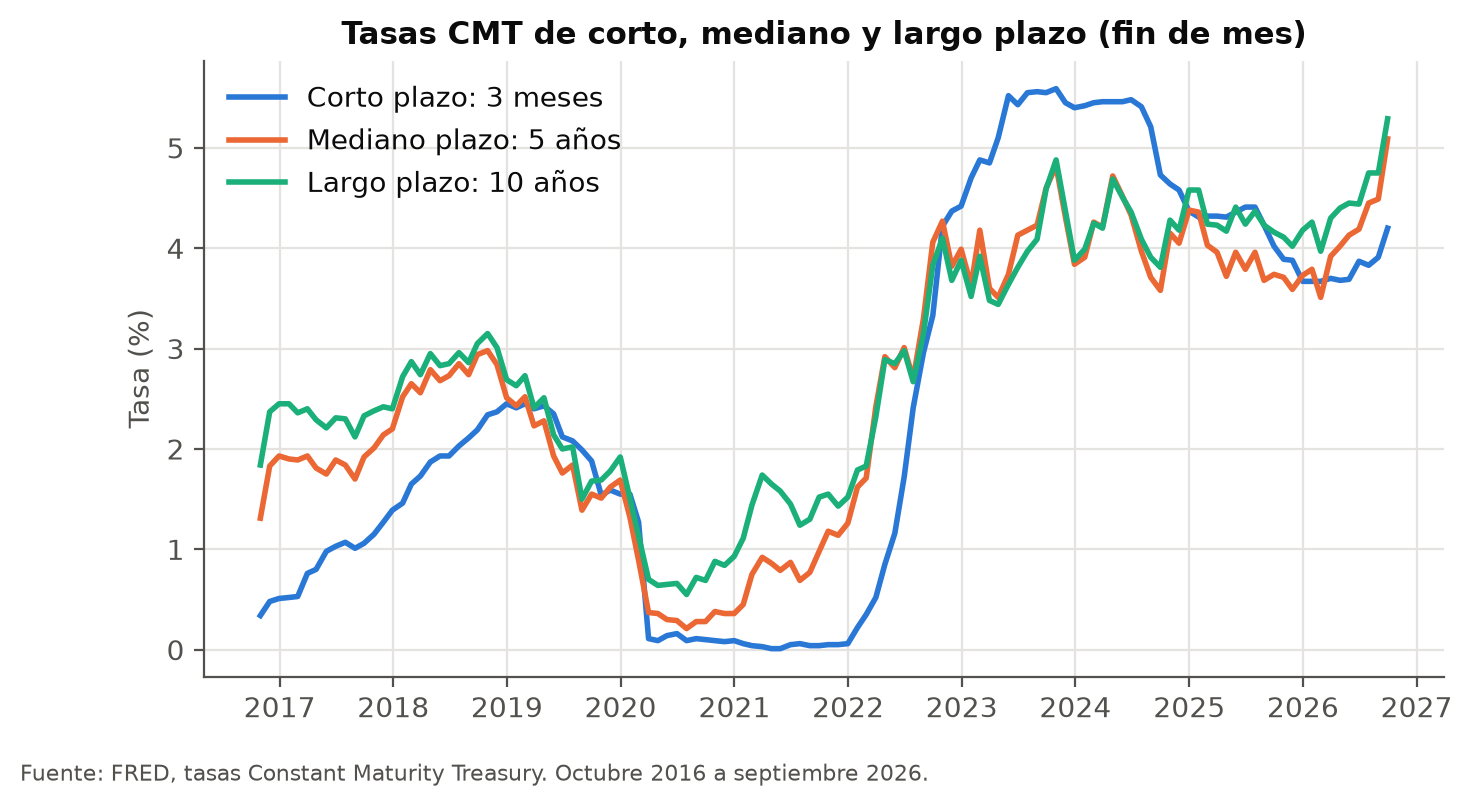
\includegraphics[width=0.85\textwidth]{p3_tasas_representativas.png}
\caption{Tasas CMT a 3 meses, 5 años y 10 años, octubre de 2016 a septiembre de 2026}
\label{fig:tasas}
\fuente{elaboración propia con datos de FRED.}
\end{figure}

\subsection{Estimación de Nelson y Siegel (preguntas 4 y 5)}

A partir de las tasas CMT se ajustó directamente la siguiente variante del modelo de Nelson y Siegel (1987):
\begin{equation}
y(m) = \beta_0 + \beta_1\,\frac{1-e^{-m/\tau}}{m/\tau}
     + \beta_2\left(\frac{1-e^{-m/\tau}}{m/\tau} - e^{-m/\tau}\right),
\label{eq:ns}
\end{equation}
En esta expresión, $m$ representa la madurez y $\tau>0$ es el parámetro de decaimiento; ambos se miden en años, mientras que $y(m)$ está expresada en porcentaje. Puesto que las CMT son rendimientos a la par, la curva estimada debe interpretarse como una curva par, no como una curva cero cupón.

Fijado un valor de $\tau$, la expresión es lineal respecto de $\beta_0$, $\beta_1$ y $\beta_2$. En consecuencia, para cada mes se estimaron esos tres coeficientes mediante mínimos cuadrados ordinarios, tomando las \MImadureces{} tasas mensuales como observaciones y manteniendo un único $\tau$ para toda la muestra. Como comprobación, al establecer $\tau = 1$ año, la suma de los SCR de las \MImeses{} regresiones mensuales es de \MIscrUno{} puntos porcentuales al cuadrado, calculada sobre \MIobs{} observaciones.

La búsqueda del $\tau$ óptimo se realizó sobre una grilla desde 0,05 hasta 15 años, con incrementos de 0,001. Para cada valor se estimaron nuevamente las \MImeses{} regresiones y se sumaron sus SCR. El menor resultado corresponde a $\tau = \MItau{}$ años, con un SCR agregado de \MIscrMin{} puntos porcentuales al cuadrado (Tabla~\ref{tab:ajuste} y Figura~\ref{fig:scr}). Dentro del intervalo evaluado, la función es continua y suave, y registra un único mínimo.

\begin{table}[H]
\centering
\caption{Ajuste del modelo de Nelson y Siegel}
\label{tab:ajuste}
\begin{tabular}{lrrr}
\toprule
Caso & $\tau$ (años) & SCR total (pp$^2$) & Observaciones \\
\midrule
\tabla{p4_p5_ajuste.tex}
\bottomrule
\end{tabular}
\fuente{elaboración propia. SCR: suma de cuadrados de los residuos de las \MImeses{} regresiones mensuales.}
\end{table}

\begin{figure}[H]
\centering
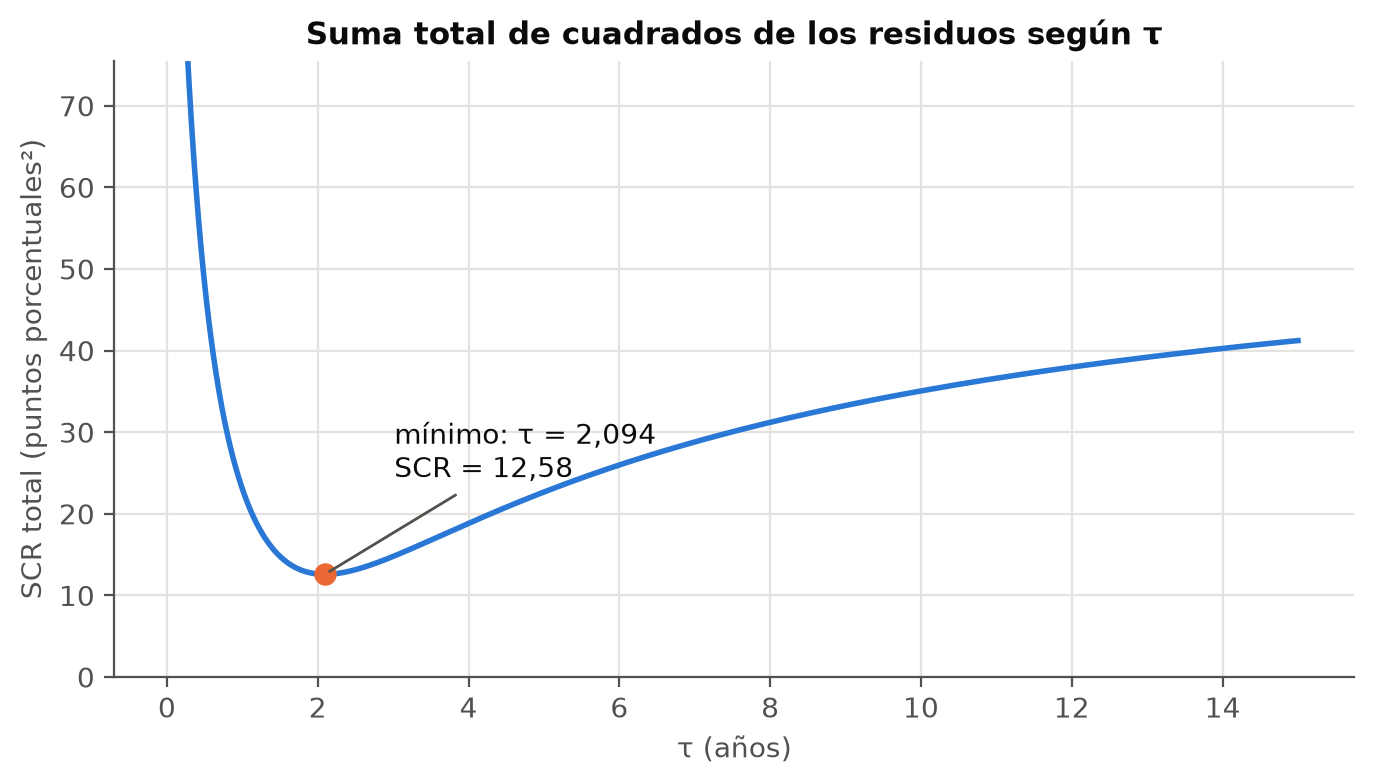
\includegraphics[width=0.8\textwidth]{p5_scr_por_tau.png}
\caption{Suma total de cuadrados de los residuos para cada valor de $\tau$}
\label{fig:scr}
\fuente{elaboración propia.}
\end{figure}

\subsection{Evolución de los parámetros (pregunta 6)}

En la Figura~\ref{fig:betas} se muestran las estimaciones de los parámetros obtenidas con el $\tau$ óptimo. Su evolución resulta consistente con la dinámica observada en las tasas:

\begin{itemize}[leftmargin=*]
\item \textbf{Nivel ($\beta_0$).} Representa el valor al que converge la curva para vencimientos largos. Alcanzó un mínimo de \MIbetaCeroMin{}\% a mediados de 2020 y, desde 2022, inició un avance persistente hasta situarse en \MIbetaCeroFin{}\% en septiembre de 2026, el máximo de toda la muestra.
\item \textbf{Pendiente ($\beta_1$).} Expresa la brecha entre la tasa instantánea de corto plazo y el nivel de largo plazo. Por ello, cuando toma valores negativos, la curva presenta pendiente positiva. El parámetro se volvió positivo entre fines de 2022 y 2024, etapa en que la curva estuvo invertida, y retornó a terreno negativo desde 2025.
\item \textbf{Curvatura ($\beta_2$).} Este coeficiente incide en los vencimientos intermedios y, con el $\tau$ estimado, alcanza su mayor efecto cerca de los 3,8 años. Es el parámetro más volátil. Su máximo se registró en abril de 2022 y coincide con el aumento anticipado de las tasas de plazo medio al inicio del ciclo de alzas de la Reserva Federal.
\end{itemize}

\begin{figure}[H]
\centering
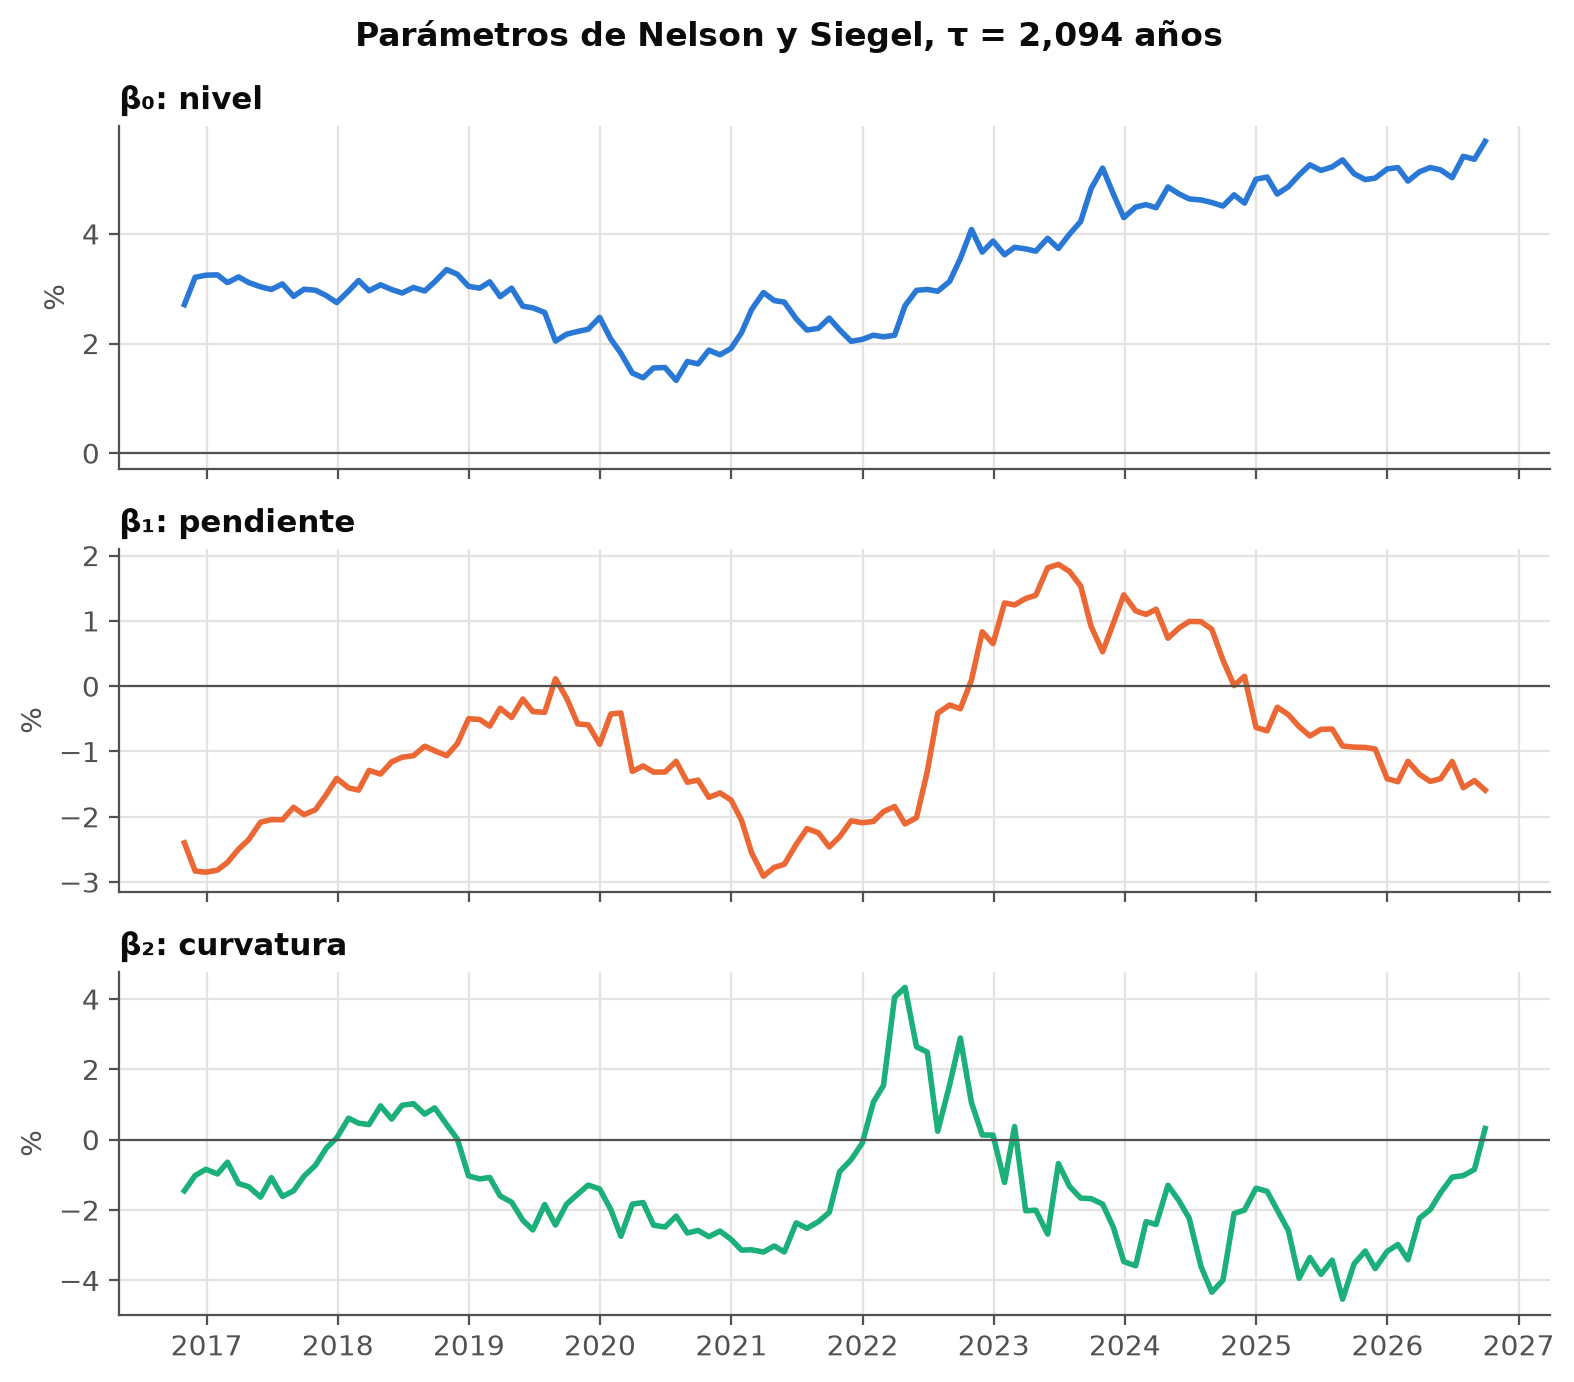
\includegraphics[width=0.85\textwidth]{p6_betas.png}
\caption{Evolución mensual de $\beta_0$, $\beta_1$ y $\beta_2$}
\label{fig:betas}
\fuente{elaboración propia.}
\end{figure}

\subsection{Comparación con la curva de la Reserva Federal (pregunta 7)}

La Figura~\ref{fig:svenpy} compara la curva estimada en este trabajo con las tasas par SVENPY publicadas por el \emph{Federal Reserve Board}, que Gürkaynak, Sack y Wright (2007) estiman mediante el modelo de Svensson (1994). Se consideran los últimos días hábiles de diciembre de 2023, diciembre de 2024, diciembre de 2025 y septiembre de 2026. Las diferencias entre ambas curvas se resumen en la Tabla~\ref{tab:svenpy}.

\begin{figure}[H]
\centering
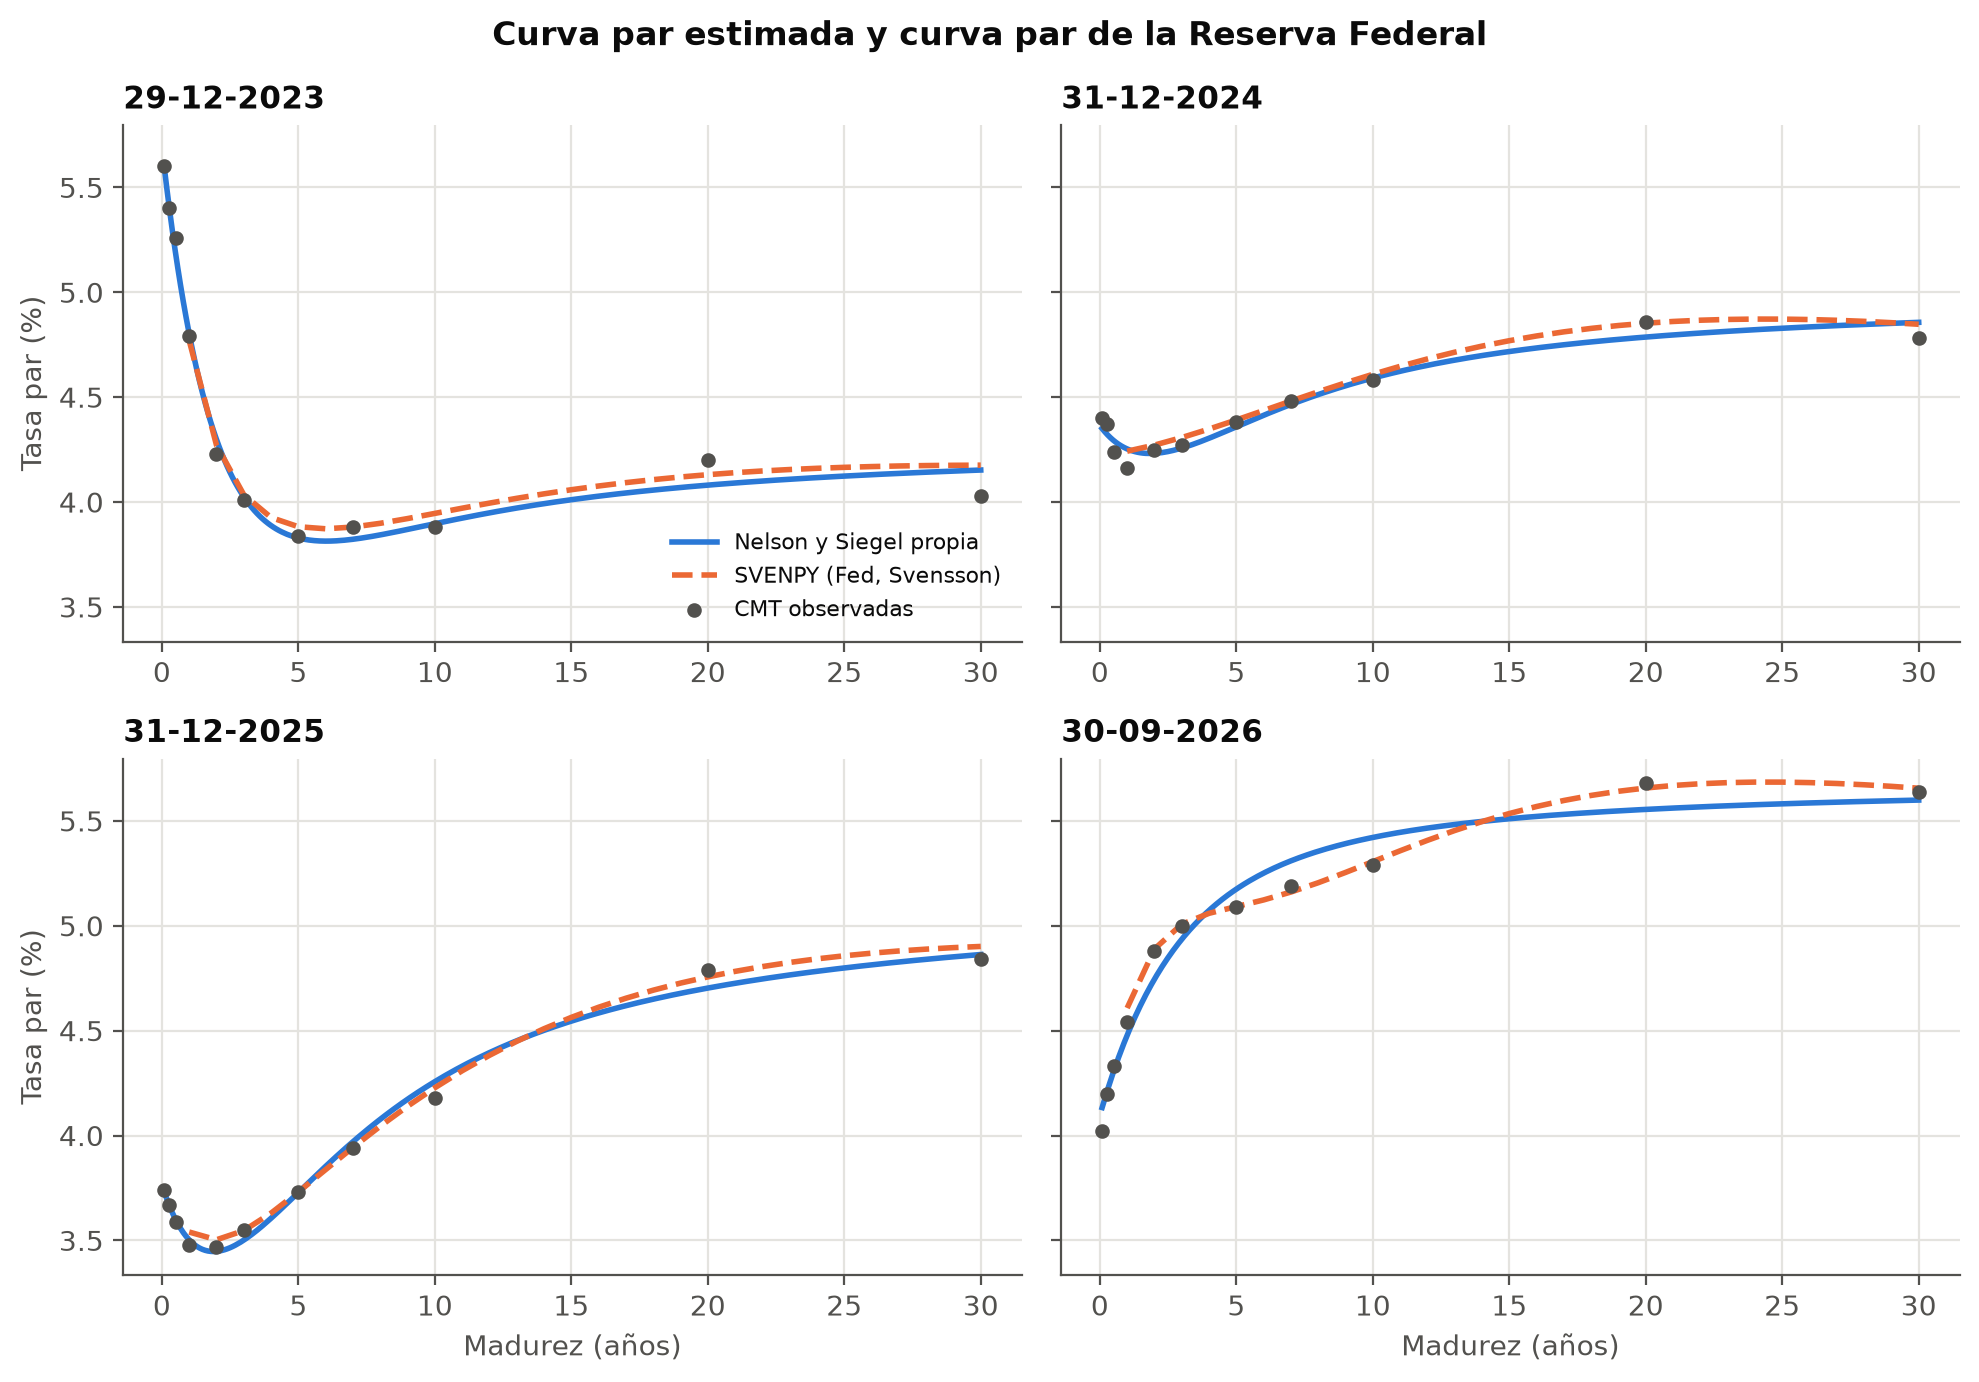
\includegraphics[width=\textwidth]{p7_comparacion_svenpy.png}
\caption{Curva par estimada y curva par SVENPY en las cuatro fechas}
\label{fig:svenpy}
\fuente{elaboración propia con datos de FRED y del Federal Reserve Board.}
\end{figure}

\begin{table}[H]
\centering
\caption{Diferencia entre la curva propia y las SVENPY (puntos base)}
\label{tab:svenpy}
\begin{tabular}{lrrrrrrr}
\toprule
 & \multicolumn{6}{c}{Madurez (años)} & Media \\
\cmidrule(lr){2-7}
Fecha & 1 & 2 & 5 & 10 & 20 & 30 & absoluta \\
\midrule
\tabla{p7_diferencias.tex}
\bottomrule
\end{tabular}
\fuente{elaboración propia. Diferencia = curva propia menos SVENPY. La media absoluta considera las 30 madureces anuales.}
\end{table}

En los tres cierres de diciembre se observa una elevada similitud entre las curvas: la diferencia absoluta promedio se aproxima a 4 puntos base y no supera los 7 puntos en ninguno de los vencimientos incluidos en la tabla. Se identifican tres diferencias principales.

\begin{itemize}[leftmargin=*]
\item \textbf{Flexibilidad.} Svensson contempla un segundo componente de curvatura y un parámetro de decaimiento propio para ese término. Además, la Reserva Federal actualiza diariamente la estimación de todos sus parámetros. El modelo utilizado aquí solo incorpora una curvatura y mantiene un $\tau$ común durante toda la muestra, lo que limita su capacidad para reproducir curvas con más de un cambio de pendiente.
\item \textbf{Septiembre de 2026.} En esta fecha se registra el ajuste menos preciso, con una diferencia promedio cercana a 9 puntos base. Para los plazos de 1 y 2 años, la curva estimada queda entre 13 y 14 puntos base por debajo de la de la Fed; a 10 años, se ubica aproximadamente 12 puntos por encima. La curva observada presenta ese día un fuerte ascenso hasta los 3 años, luego se aplana entre 3 y 10 años y vuelve a subir hacia los 20 años. Una única curvatura no permite reproducir adecuadamente esa configuración.
\item \textbf{Datos de origen.} La estimación propia utiliza 11 tasas CMT, que ya constituyen una interpolación basada en los títulos más recientes, e incluye las letras de corto plazo. En cambio, la Reserva Federal estima su curva a partir de los precios de un conjunto más amplio de notas y bonos, sin incorporar letras ni las emisiones más recientes.
\end{itemize}

La diferencia observada en septiembre de 2026 es relevante para las secciones siguientes, ya que esa misma curva se emplea en el módulo III para calcular el valor de los swaps al cierre del período. Esta circunstancia se considera una limitación del análisis y se retoma al discutir los resultados.

% --------------------------------------------------------------- Módulo II
\section{Módulo II: montos vigentes en swaps de tasas de interés en dólares}

\subsection{AFP asignada, patrimonio y rentabilidad (pregunta 8)}

Los dígitos verificadores de los RUT de quienes integran el grupo son 5, 7 y 9. La suma es 21 y, dado que $21 \bmod 7 = 0$, la asignación correspondiente es el Fondo E de AFP Capital.

La información del valor cuota y del patrimonio se obtuvo desde el sitio de la Superintendencia de Pensiones para el 31 de diciembre de 2025 y para el último día de cada mes entre enero y septiembre de 2026. Todas las observaciones corresponden a valores confirmados. La rentabilidad nominal mensual se determinó mediante la variación porcentual del valor cuota, mientras que la rentabilidad real se obtuvo ajustando ese resultado por la variación de la UF en el mismo lapso:
\[
1 + r_t^{\text{real}} = \frac{1 + r_t^{\text{nominal}}}{\text{UF}_t/\text{UF}_{t-1}}.
\]
Los datos de la UF se extrajeron del apartado ``Valores monetarios'' de la Superintendencia de Pensiones, que reproduce las cifras diarias publicadas por el Banco Central de Chile.

\begin{table}[H]
\centering
\caption{Fondo E de AFP Capital: valor cuota, patrimonio y rentabilidades}
\label{tab:rent}
\small
\begin{tabular}{lrrrrrrr}
\toprule
 & Valor cuota & Patrimonio & UF & \multicolumn{2}{c}{Rent.\ mensual} & \multicolumn{2}{c}{Rent.\ acumulada} \\
\cmidrule(lr){5-6}\cmidrule(lr){7-8}
Fecha & (\$) & (MMM\$) & (\$) & Nominal & Real & Nominal & Real \\
\midrule
\tabla{p8_tabla.tex}
\bottomrule
\end{tabular}
\fuente{elaboración propia con datos de la Superintendencia de Pensiones. MMM\$: miles de millones de pesos. Rentabilidad acumulada desde el 31-12-2025.}
\end{table}

En el lapso entre diciembre de 2025 y septiembre de 2026, el fondo acumuló una rentabilidad nominal de \MIInominal{}. Al incorporar el aumento de \MIIuf{} de la UF, la rentabilidad real llegó a \MIIreal{} (Tabla~\ref{tab:rent} y Figura~\ref{fig:rentacum}). Frente al promedio de $-$10,39\% del sistema señalado en la introducción, el resultado de AFP Capital fue ligeramente peor. El retroceso se produjo principalmente durante la segunda mitad del período; \MIIpeorMes{} fue el mes más negativo, con una rentabilidad nominal de \MIIpeorMesRent{}. Por su parte, el patrimonio pasó de \MIIpatIni{} a \MIIpatFin{} billones de pesos (\MIIpatVar{}). Esta contracción, superior a la caída del valor cuota, sugiere que también se registraron retiros netos de recursos del fondo (Figura~\ref{fig:pat}).

\begin{figure}[H]
\centering
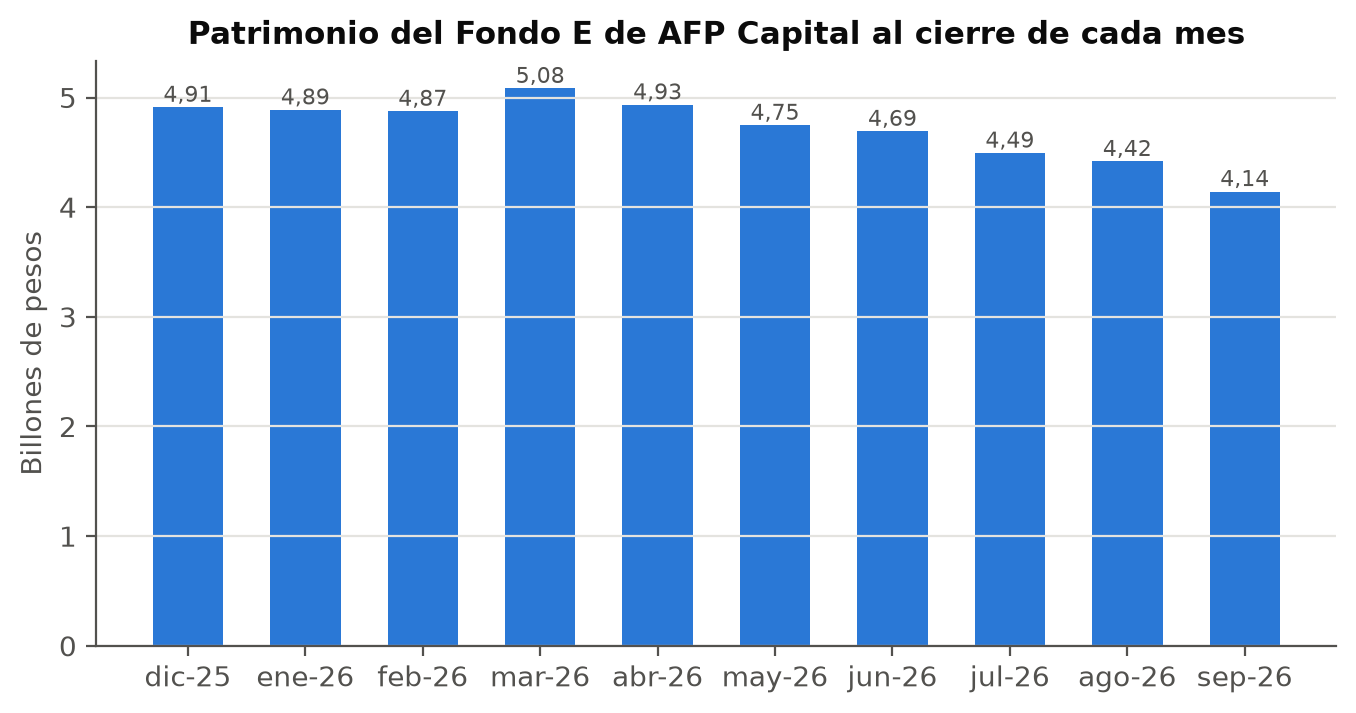
\includegraphics[width=0.8\textwidth]{p8_patrimonio.png}
\caption{Patrimonio del Fondo E de AFP Capital al cierre de cada mes}
\label{fig:pat}
\fuente{elaboración propia con datos de la Superintendencia de Pensiones. Un billón equivale a $10^{12}$ pesos.}
\end{figure}

\begin{figure}[H]
\centering
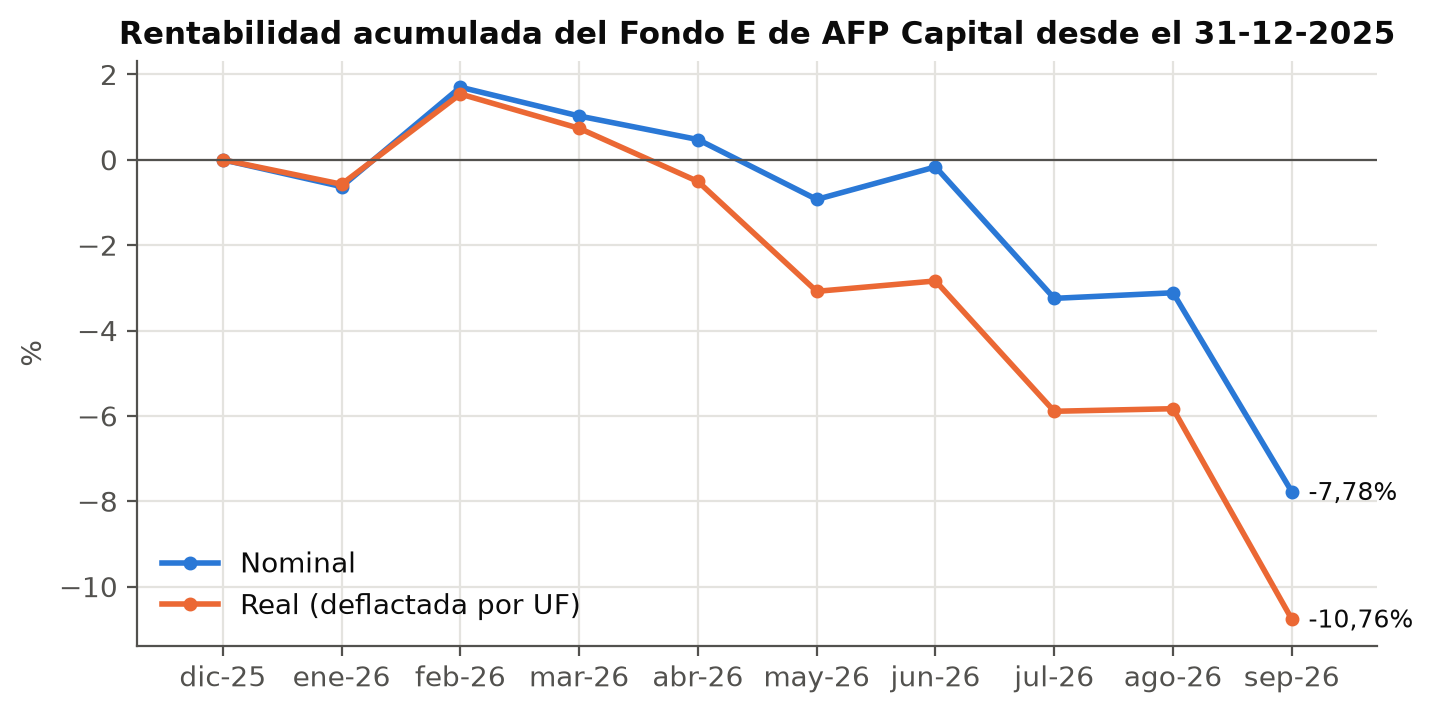
\includegraphics[width=0.8\textwidth]{p8_rentabilidad_acumulada.png}
\caption{Rentabilidad acumulada nominal y real desde el 31 de diciembre de 2025}
\label{fig:rentacum}
\fuente{elaboración propia con datos de la Superintendencia de Pensiones.}
\end{figure}

\subsection{Derivados de los Fondos de Pensiones según el SIID (pregunta 9)}

El Monitor de Derivados del SIID informa los montos vigentes al cierre mensual para el conjunto de los Fondos de Pensiones. Las cifras corresponden a nocionales ---la base sobre la que se determinan los pagos de intereses--- y no al valor de mercado de los contratos. Como están expresadas en millones de dólares de Estados Unidos, no requieren conversión monetaria. Las series se obtuvieron de la Base de Datos Estadísticos del Banco Central, que reproduce las mismas estadísticas del Monitor, debido a que, al momento de la descarga, los archivos Excel disponibles en este último solo llegaban hasta abril de 2026.

La Figura~\ref{fig:siid} expone los montos vigentes por subyacente desde \MIIsiidDesde{}. En septiembre de 2026, el total alcanza \MIIsiidTotal{} miles de millones de dólares; de ese monto, \MIIsiidExt{} (\MIIsiidExtPart{}) corresponden a swaps de tasas de interés extranjeras. Esta clase de instrumentos explica prácticamente la totalidad del crecimiento registrado durante el período, pues tres años antes alcanzaba \MIIsiidExtIni{} miles de millones.

\begin{figure}[H]
\centering
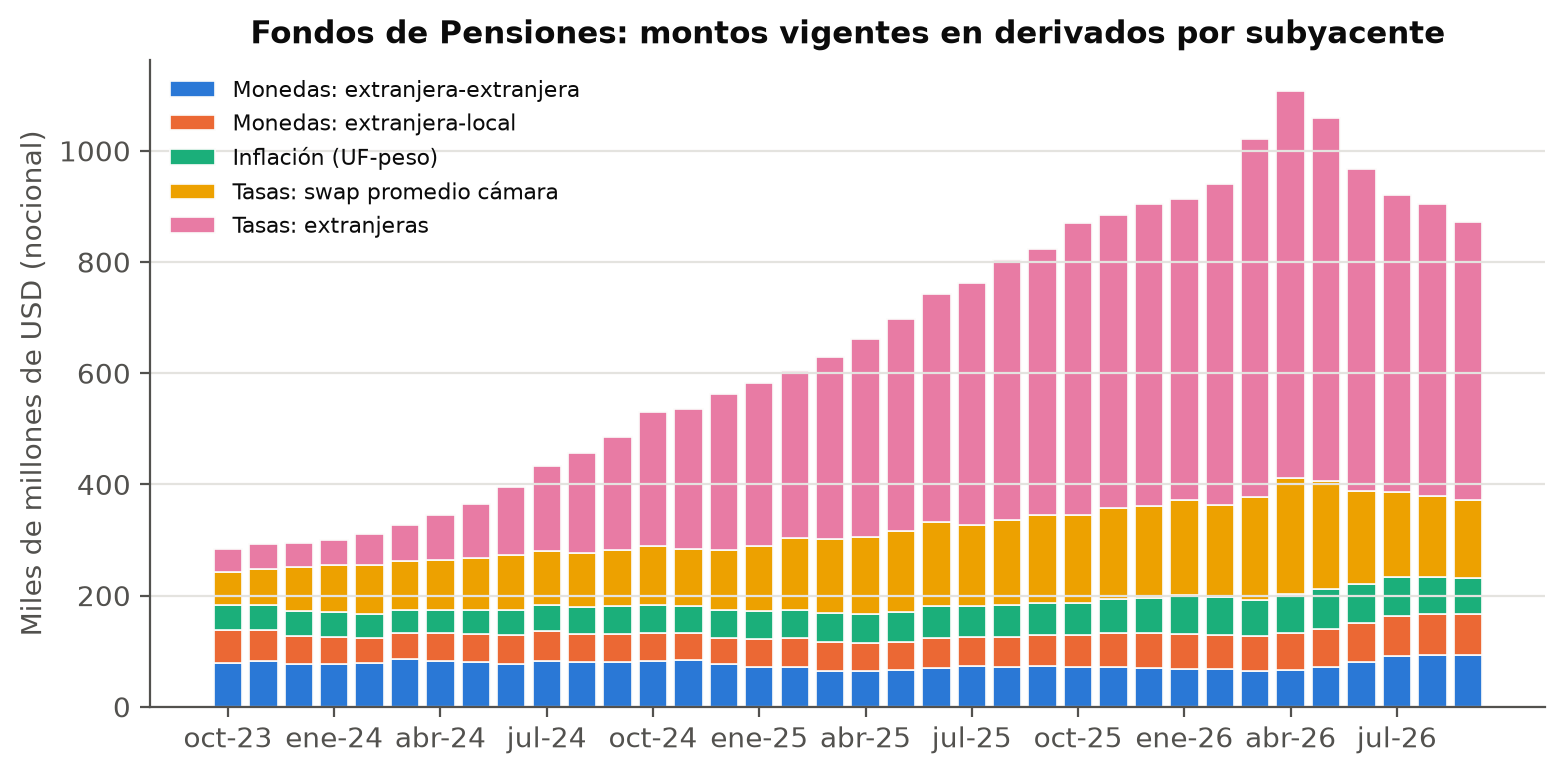
\includegraphics[width=0.9\textwidth]{p9_siid_subyacente.png}
\caption{Fondos de Pensiones: montos vigentes totales en derivados por tipo de subyacente}
\label{fig:siid}
\fuente{elaboración propia con datos del SIID, Banco Central de Chile (cuadro DER\_RES\_POS\_02 de la BDE).}
\end{figure}

En la Figura~\ref{fig:siidswaps} se presenta el detalle de los swaps de tasas extranjeras. El SIID clasifica las operaciones según la tasa variable: cuando se vende tasa variable, el fondo paga una tasa flotante y recibe una fija (compra fija); cuando se compra tasa variable, paga fija y recibe flotante (venta fija). Hasta marzo de 2026, ambos sentidos crecieron a un ritmo muy parecido. El monto total llegó a su punto máximo en abril de 2026, con \MIIsiidExtMax{} miles de millones, y desde entonces las compras de tasa variable cayeron a menos de la mitad, mientras las ventas se mantuvieron.

\begin{figure}[H]
\centering
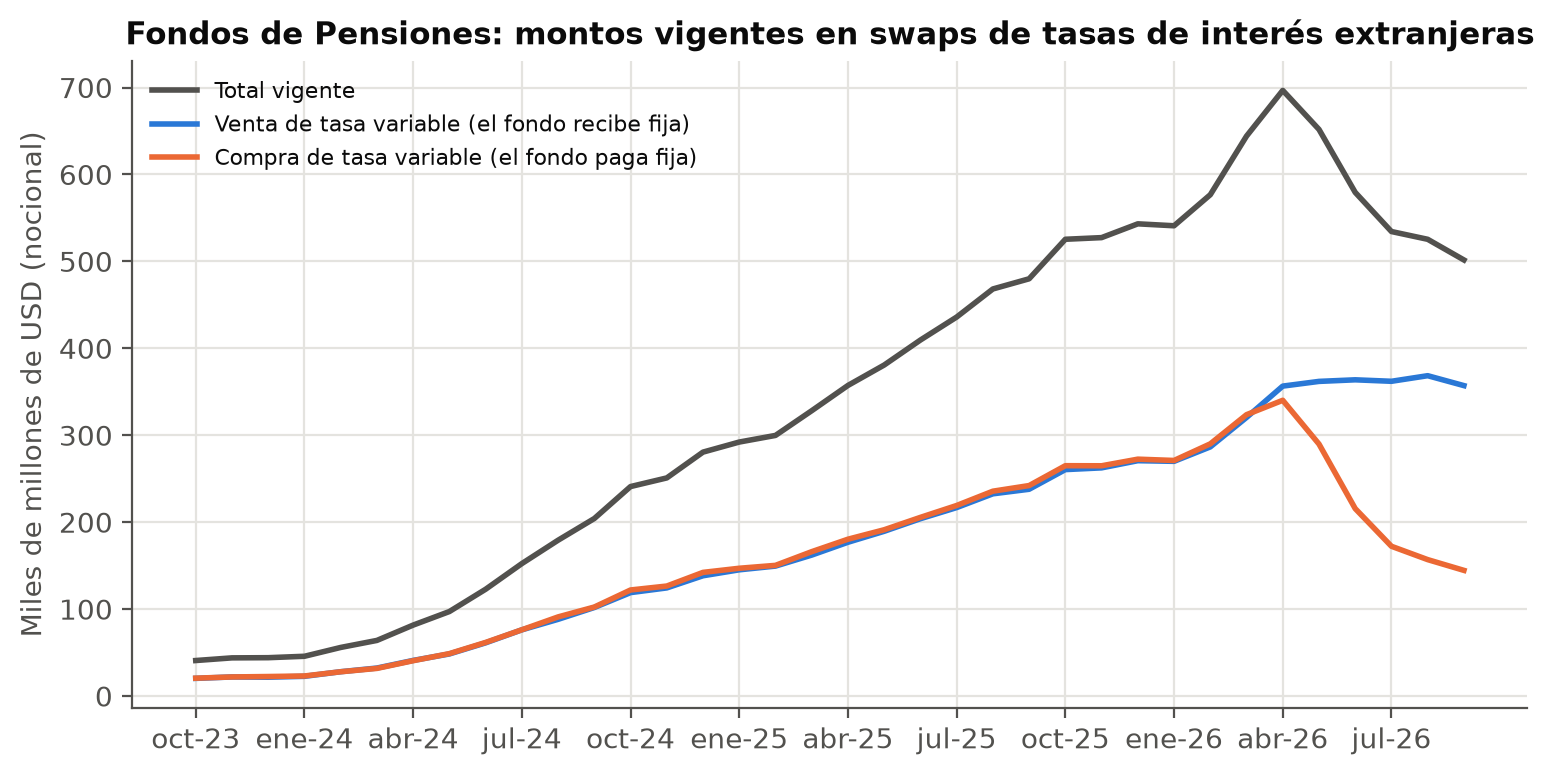
\includegraphics[width=0.9\textwidth]{p9_siid_swaps_extranjeros.png}
\caption{Fondos de Pensiones: montos vigentes en swaps de tasas de interés extranjeras}
\label{fig:siidswaps}
\fuente{elaboración propia con datos del SIID, Banco Central de Chile (cuadro DER\_TAS\_FP\_STO\_01 de la BDE).}
\end{figure}

\subsection{Carteras históricas y variables de los swaps (pregunta 10)}

Las posiciones del fondo se extrajeron de los archivos de carteras históricas de inversión publicados por la Superintendencia de Pensiones. Estos archivos registran cada instrumento, fondo y fecha de cierre mensual. Se filtraron las observaciones del Fondo E de AFP Capital cuyas tasas pactadas incluyen el descriptor \texttt{SFRUS\$360}, correspondiente a la tasa SOFR denominada en dólares.

Cada swap aparece con dos tasas:
\begin{itemize}[leftmargin=*]
\item \texttt{tasa\_pactada\_del\_fondo\_swap}: corresponde al interés que el Fondo de Pensiones acuerda pagar sobre el capital.
\item \texttt{tasa\_pactada\_de\_la\_contraparte\_swap}: representa la tasa que paga la contraparte y que, por tanto, recibe el fondo.
\end{itemize}
En cada registro, una de las tasas corresponde a SOFR sin \emph{spread} (\texttt{SFRUS\$360+00,0000ACT/360}), mientras que la otra es una tasa fija en dólares (por ejemplo, \texttt{FIJAUS\$+03,8250ACT/360}, equivalente a un 3,825\% anual con base ACT/360). La combinación de ambas permite identificar el sentido del swap: si el fondo tiene pactada SOFR y la contraparte una tasa fija, el fondo recibe fija y paga flotante (compra fija); si el fondo tiene la tasa fija, paga fija y recibe flotante (venta fija). La variable \texttt{unidades} contiene el nocional en dólares, y el nemotécnico identifica a la contraparte, el vencimiento y la fecha de inicio del contrato.

\subsection{Posiciones observadas en las carteras (pregunta 11)}

Con esos registros se construyó una serie mensual de posiciones que comienza en enero de 2024 y llega hasta la cartera más reciente disponible. Se tomó como cartera base la correspondiente a junio de 2026, con fecha de cierre \MIIbaseFecha{}. La base completa incluye las columnas Mes, Año de madurez, Nocional compra fija, Nocional venta fija y Neto compra fija, y está guardada en \texttt{output/tablas/p11\_posiciones\_observadas.csv}. La Tabla~\ref{tab:base} contiene la cartera base y la Tabla~\ref{tab:totales} presenta los totales de cada mes.

\begin{table}[H]
\centering
\caption{Cartera base (\MIIbase): nocional por año de madurez, en millones de USD}
\label{tab:base}
\begin{tabular}{lrrr}
\toprule
Año de madurez & Compra fija & Venta fija & Neto compra fija \\
\midrule
\tabla{p11_base_por_anio.tex}
\bottomrule
\end{tabular}
\fuente{elaboración propia con las carteras de la Superintendencia de Pensiones.}
\end{table}

La cartera base está compuesta por \MIIcontratosBase{} contratos. El fondo mantiene \MIIcompraBase{} millones de dólares en compra fija y \MIIventaBase{} millones en venta fija, con una posición neta de \MIInetoBase{} millones. Como referencia, el patrimonio del fondo equivalía entonces a \MIIpatBaseUsd{} miles de millones de dólares; por consiguiente, el nocional de compra fija era \MIIcompraSobrePat{} veces dicho patrimonio. Los vencimientos de ambos lados presentan perfiles muy distintos. La compra fija vence entre 2029 y 2045, tiene un plazo residual promedio de \MIIresCompra{} años y una tasa fija media de \MIItasaCompra{}\%. La venta fija, por el contrario, se concentra en contratos con vencimiento durante 2026: el \MIIpesoVentaCorto{} del nocional corresponde al tramo de 3 meses y su tasa promedio es \MIItasaVenta{}\%.

\subsection{Tabla completada con el SIID (pregunta 12)}

Dado que aún no estaban disponibles las carteras de julio, agosto y septiembre de 2026, fue necesario estimar las posiciones de esos meses. Para ello se supuso que los nocionales de compra fija y venta fija del fondo evolucionan, de manera independiente, en la misma proporción que sus respectivos agregados del SIID, tomando como punto de partida la cartera base:
\[
N^{s}_{t} = N^{s}_{\text{base}} \times \frac{\text{SIID}^{s}_{t}}{\text{SIID}^{s}_{\text{base}}},
\qquad s \in \{\text{compra fija},\ \text{venta fija}\},
\]
El agregado de compra fija se asocia a la venta de tasa variable informada por el SIID, mientras que el agregado de venta fija corresponde a la compra de tasa variable. Este procedimiento supone, en términos prácticos, que la proporción que representa el fondo dentro de cada agregado permanece constante. También se mantienen, para cada sentido de la operación, la distribución por año de madurez y tramo de plazo, las duraciones y las tasas fijas pactadas de la cartera base. La posición neta se obtiene restando las ventas a las compras. La Tabla~\ref{tab:factores} muestra los factores utilizados.

\begin{table}[H]
\centering
\caption{Agregados del SIID usados en la extrapolación}
\label{tab:factores}
\begin{tabular}{lrrrr}
\toprule
 & \multicolumn{2}{c}{Compra fija (venta variable)} & \multicolumn{2}{c}{Venta fija (compra variable)} \\
\cmidrule(lr){2-3}\cmidrule(lr){4-5}
Mes & MMM USD & Factor & MMM USD & Factor \\
\midrule
\tabla{p12_factores_siid.tex}
\bottomrule
\end{tabular}
\fuente{SIID, Banco Central de Chile (BDE, cuadro DER\_TAS\_FP\_STO\_01), descargado el 15-11-2026. MMM USD: miles de millones de dólares. Factor respecto de la cartera base.}
\end{table}

\begin{table}[H]
\centering
\caption{Fondo E de AFP Capital: nocional total en swaps SOFR por mes, en millones de USD}
\label{tab:totales}
\small
\begin{tabular}{lrrrrl}
\toprule
Mes & Compra fija & Venta fija & Neto compra fija & Contratos & Origen \\
\midrule
\tabla{p12_totales_mensuales.tex}
\bottomrule
\end{tabular}
\fuente{elaboración propia. Carteras de la Superintendencia de Pensiones (descargadas el 15-11-2026, cartera base de \MIIbase) y agregados del SIID. El detalle por año de madurez, con la columna Origen, está en \texttt{output/tablas/p12\_posiciones\_completadas.csv}.}
\end{table}

Para evaluar si el supuesto de proporcionalidad resulta adecuado, se contrastó con la trayectoria histórica del fondo (Figura~\ref{fig:prop}). El análisis indica que puede utilizarse como una aproximación inicial, pero no como una estimación precisa.

\begin{itemize}[leftmargin=*]
\item \textbf{Participaciones.} En los doce meses previos a la cartera base, la proporción del fondo dentro del agregado de compra fija fluctuó entre \MIIpartCompraMin{} y \MIIpartCompraMax{}; en el agregado de venta fija, se ubicó entre \MIIpartVentaMin{} y \MIIpartVentaMax{}. No aparece una tendencia clara, aunque sí se observan variaciones puntuales en agosto y noviembre de 2025, cuando el fondo abrió y cerró posiciones de corto plazo en ambos sentidos.
\item \textbf{Error histórico.} Si se hubiese utilizado anteriormente el mismo criterio, el error absoluto promedio para horizontes de uno y tres meses habría alcanzado \MIIerrCompraUno{} y \MIIerrCompraTres{} en compra fija, y \MIIerrVentaUno{} y \MIIerrVentaTres{} en venta fija, respectivamente. Los valores corresponden a los promedios de los últimos doce meses observados.
\item \textbf{Composición por plazo.} La compra fija se ha concentrado de forma persistente en los tramos de 5 y 10 años, que representaban \MIIpesoCompraLargo{} de la cartera base. Sin embargo, durante 2026 el tramo de 2 años ha ganado peso a medida que los contratos se aproximan al vencimiento. Mantener sin cambios la composición de junio no captura ese envejecimiento ni los vencimientos de la venta fija, cuyo plazo es reducido.
\end{itemize}

La hipótesis presenta su mayor debilidad justamente durante los meses para los que se aplica. Desde abril de 2026, la venta fija del fondo cae con mayor rapidez que la del sistema y su participación desciende a \MIIpartVenta{} en junio. Por esta razón, la extrapolación podría sobrestimar la venta fija que continúa vigente. En consecuencia, las cifras de julio a septiembre deben leerse como estimaciones.

\begin{figure}[H]
\centering
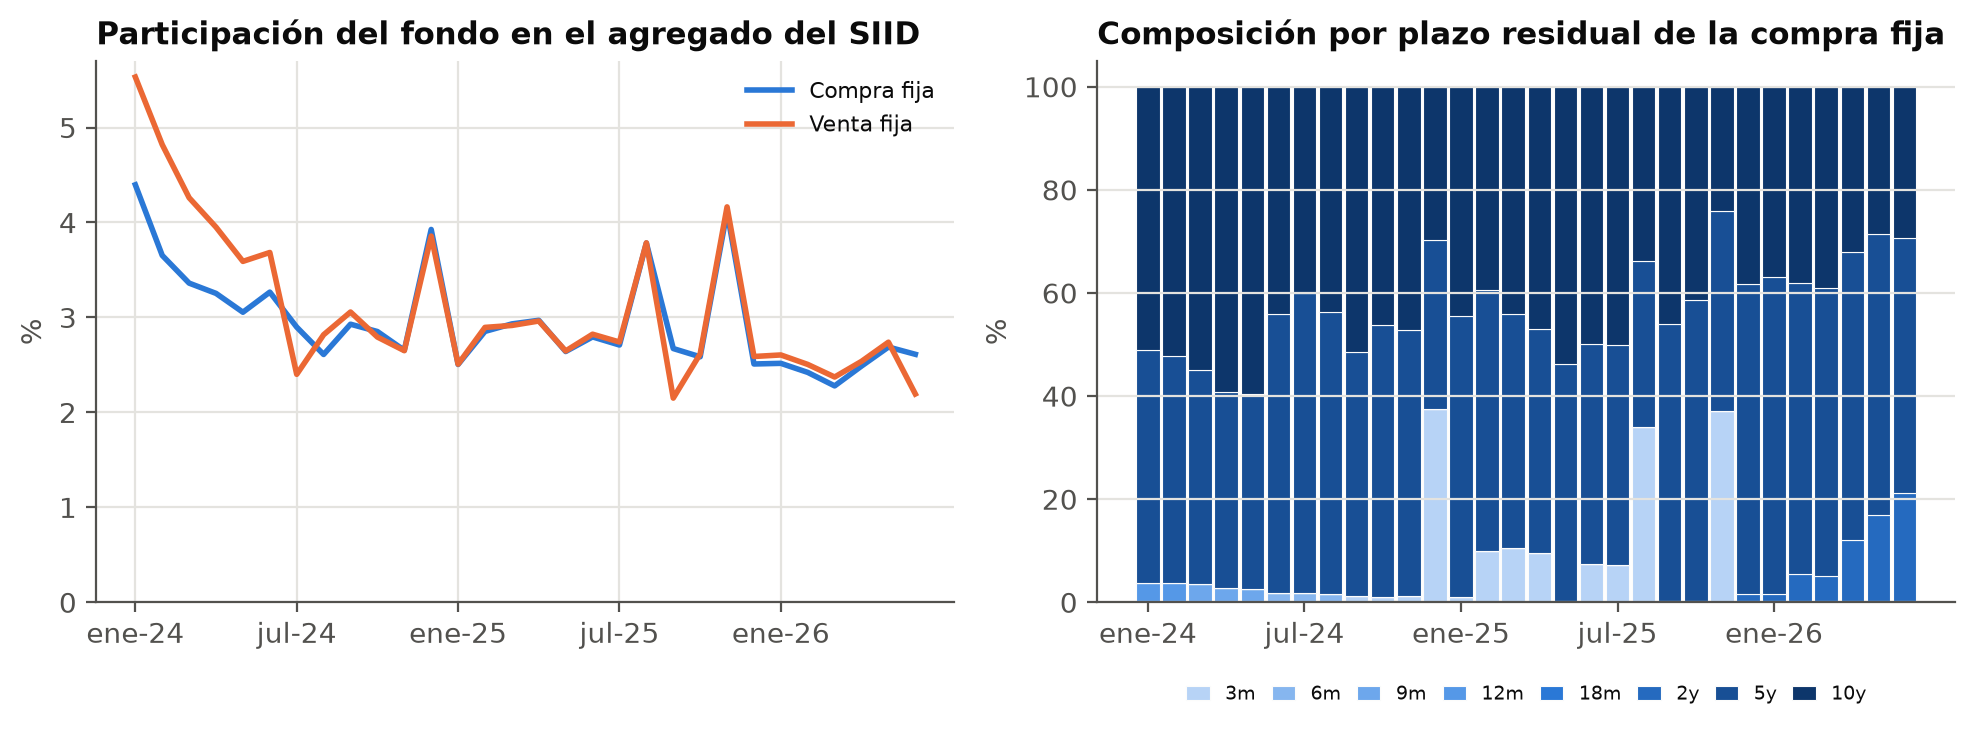
\includegraphics[width=\textwidth]{p12_proporcionalidad.png}
\caption{Participación del fondo en los agregados del SIID y composición por plazo de la compra fija}
\label{fig:prop}
\fuente{elaboración propia con las carteras de la Superintendencia de Pensiones y el SIID.}
\end{figure}

\subsection{Evolución de las posiciones por plazo (pregunta 13)}

La Figura~\ref{fig:tramos} reúne las posiciones observadas y estimadas, clasificadas por plazo residual. Para cada swap se determinó el tiempo entre la fecha de la cartera y su vencimiento, y luego se asignó al tramo más próximo entre 3, 6, 9, 12 y 18 meses, y 2, 5 y 10 años. Si existía un empate, se asignó el tramo de mayor duración. Los totales mensuales son los mismos que aparecen en la Tabla~\ref{tab:totales}.

\begin{figure}[H]
\centering
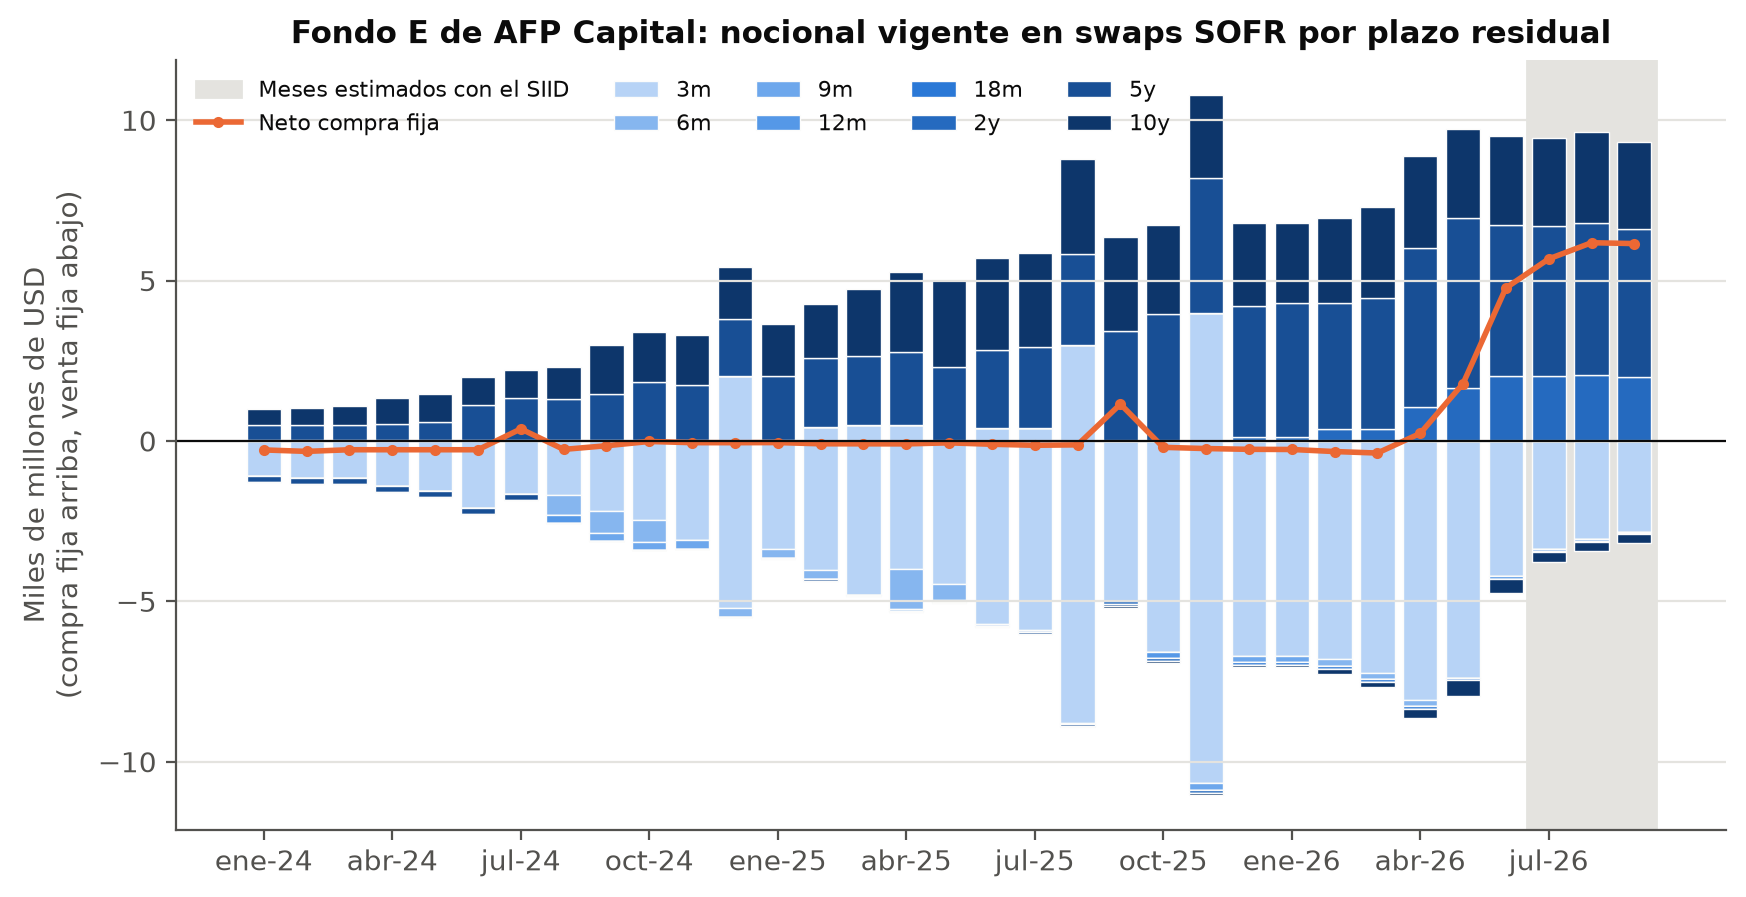
\includegraphics[width=\textwidth]{p13_posiciones_por_tramo.png}
\caption{Fondo E de AFP Capital: nocional vigente en swaps SOFR, compra y venta de tasa fija por plazo residual}
\label{fig:tramos}
\fuente{elaboración propia. Barras positivas: compra fija; negativas: venta fija. Zona gris: meses estimados con los agregados del SIID y las ponderaciones de \MIIbase.}
\end{figure}

Hasta marzo de 2026, las posiciones nocionales del fondo estaban casi equilibradas: la compra fija se ubicaba en vencimientos largos (5 y 10 años), mientras que la venta fija se concentraba en plazos muy breves (3 meses). El saldo neto era cercano a cero (\MIInetoMar{} millones en marzo). Desde abril, la venta fija deja de renovarse y el neto sube a \MIInetoBase{} millones en junio y, según las estimaciones, a \MIInetoFin{} millones en septiembre. Un nocional neto próximo a cero no significa que la posición estuviera cubierta, porque los vencimientos de ambos lados difieren considerablemente y, por ello, también difiere su sensibilidad a las tasas. El módulo III desarrolla este punto.

\subsection{Contrapartes (pregunta 14)}

\begin{table}[H]
\centering
\caption{Contrapartes de los swaps SOFR del Fondo E de AFP Capital al \MIIbaseFecha, en millones de USD}
\label{tab:contrapartes}
\footnotesize
\begin{tabular}{llrrrr}
\toprule
Contraparte & Origen & Compra fija & Venta fija & Bruto & Participación \\
\midrule
\tabla{p14_contrapartes.tex}
\bottomrule
\end{tabular}
\fuente{elaboración propia con la cartera de \MIIbase{} de la Superintendencia de Pensiones. Nocional bruto: compra más venta.}
\end{table}

El fondo opera con \MIIcontrapartes{} contrapartes (Tabla~\ref{tab:contrapartes}). En el otro extremo de las operaciones se encuentran, prácticamente en todos los casos, grandes entidades bancarias internacionales que actúan como intermediarias de derivados. Se trata de bancos de inversión y bancos universales de Estados Unidos, Francia y el Reino Unido, que concentran el \MIIextranjeras{} del nocional bruto. Las instituciones locales ---Itaú, Santander y Scotiabank en Chile--- tienen una participación menor y solo intervienen en operaciones de compra fija.

La cartera presenta una concentración elevada. La contraparte de mayor tamaño reúne el \MIItopUno{} del nocional bruto; las tres principales concentran el \MIItopTres{} y las cinco primeras, el \MIItopCinco{}. El índice Herfindahl-Hirschman, calculado sobre el nocional bruto, es de \MIIhhi{} puntos, cifra que suele asociarse a una concentración entre moderada y alta. De todos modos, el nocional bruto no mide directamente el riesgo de crédito con cada contraparte, pues este depende del valor de mercado de los contratos y de las garantías intercambiadas.


\end{document}
